\section{Événements utilisés}\label{chapter-ML-section-evt_gen}
%Utiliser les mêmes données simulées que dans les analyses de physique afin d'entraîner les modèles introduirait un biais.
L'objectif des modèles à entraîner est de reconstruire la masse des particules se désintégrant en paire de leptons tau.
Il s'agit d'une tâche de régression, il faut donc entraîner les modèles sur le plus de valeurs différentes possible.
Dans l'optique d'une utilisation dans les analyses telles que celle présentée dans le chapitre~\refChHTT,
il a été choisi d'utiliser des événements
$\higgsML\to\tau\tau$
où \higgsML\ est le boson de Higgs du modèle standard \higgs\ dont la masse est modifiée.
La cible du modèle est donc la masse $m_{\higgsML}$.
\subsection{Génération avec \FASTSIM}\label{chapter-ML-section-evt_gen-FASTSIM}
Nous avons généré nos propres données simulées~\cite{fastsim_ece}
afin d'obtenir des événements indépendants de ceux utilisés dans les analyses.
Dans le contexte de la collaboration CMS, nous avons utilisé \FASTSIM~\cite{FastSim_2011,FastSim_2014,FastSim_2017_1,FastSim_2017_2}.
Cet outil permet de procéder à l'ensemble de la simulation des événements introduite chapitre~\refChLHCCMS,
de la génération du processus physique à la reconstruction des objets physiques par le détecteur.
\par
Les processus physiques sont générés par
\PYTHIA~8~\cite{pythia8.2}
avec les réglages CUEP8M1~\cite{tunes_2016,tunes_2019}.
L'énergie dans le centre de masse est de \SI{13}{\TeV}.
Pour ne pas générer d'événements indésirables,
seules les collisions créant un boson de Higgs par fusion de gluons, mode dominant pour le modèle standard, sont autorisées.
De plus, le rapport de branchement $\BR(\higgsML\to\tau\tau)$ est fixé à 1,
\ie\ que \higgsML\ se désintègre forcément en paires de leptons taus.
\begin{wrapfigure}{R}{.45\textwidth}
\centering
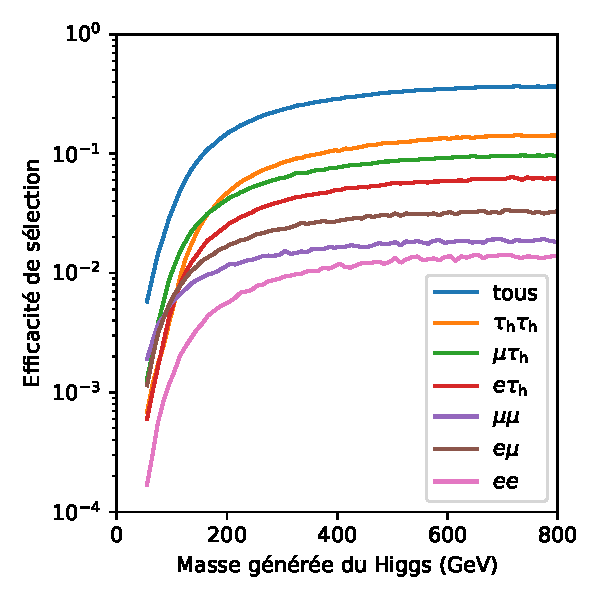
\includegraphics[width=.45\textwidth]{\PhDthesisdir/plots_and_images/my_plots/ML/from_ML_plots/FastSim_NanoAOD_to_NN/ALL_PU2017/plots_Htt_merged_NanoAODSIM_ALL_PU2017-DeepTau_1000/analysis_cuts_efficiency.pdf}
\caption[Efficacité de sélection des événements.]{Efficacité de sélection des événements pour $m_{\higgsML}\in\llbracket \num{50} , \num{800} \rrbracket \usp \SI{}{\GeV}$ dans les différents canaux et pour tous les canaux.}
\label{fig-analysis_cuts_efficiency}
\end{wrapfigure}
\par
La masse de \higgsML\ varie de \num{50} à \SI{800}{\GeV} par pas de \SI{1}{\GeV}.
Il est important d'utiliser l'intervalle le plus étendu possible, il correspond à la gamme utile des modèles obtenus.
L'effet de l'étendue de cet intervalle est discuté dans la section~\ref{chapter-ML-section-discussion}.
Lorsque $m_{\higgsML}$ est supérieure à \SI{800}{\GeV}, les propriétés de \higgsML, basées sur celles de \higgs, ne permettent pas d'obtenir des valeurs de $m_{\higgsML}$ cohérentes avec la méthode de génération utilisée.
Nous ne considérerons pas de masse plus haute.
Bien qu'il soit possible pour une particule de se désintégrer en deux taus dès que sa masse est plus élevée que $2\,m_{\tau} = \SI{3.5}{\GeV}$,
la sélection des événements présentée dans la section~\ref{chapter-ML-section-evt_gen-selection} rejette plus de \SI{99}{\%} des événements lorsque $m_{\higgsML} < \SI{50}{\GeV}$.
Nous ne considérerons pas de masse plus basse.
L'efficacité des sélections appliquées est représentée sur la figure~\ref{fig-analysis_cuts_efficiency}.
S'il est possible d'appliquer des poids aux événements afin d'équilibrer l'entraînement sur l'ensemble des valeurs de la cible,
plus d'événements sont générés à basse masse afin d'obtenir des topologies d'événements variées malgré la faible efficacité de sélection.
Ainsi, la quantité d'événements générés pour chaque valeur de $m_{\higgsML}$ est de:
\begin{itemize}
\item \num{60000} pour $ \num{50} \geq m_{\higgsML} < \num{300} $;
\item \num{20000} pour $ \num{300} \geq m_{\higgsML} < \num{500} $;
\item \num{10000} pour $ \num{500} \geq m_{\higgsML} \geq \num{800}$.
\end{itemize}
\par
L'empilement est modélisé par superposition du signal $\higgsML\to\tau\tau$ à des événements dits de \og biais minimum \fg~\cite{pythia8.2}.
Il s'agit d'événements pouvant contenir des interactions dures, mais n'activant pas de \HLTpath.
La quantité d'empilement ajoutée à l'événement $\higgsML\to\tau\tau$ suit le profil de l'année 2017.
\subsection{Sélection des événements}\label{chapter-ML-section-evt_gen-selection}
\subsubsection{Canaux \tauh\tauh, \mu\tauh, \ele\tauh\ et \ele\mu}
La sélection des événements se fait comme exposé dans le chapitre~\refChHTT\ pour l'année 2017 et les canaux
\tauh\tauh, \mu\tauh, \ele\tauh\ et \ele\mu\ y étant exploités,
à l'exception des coupures servant à séparer la région de signal des régions de contrôle et de détermination, sur
$\mT^{(\mu)}$ dans le canal \mu\tauh,
$\mT^{(\ele)}$ dans le canal \ele\tauh,
$\Dzeta$ dans le canal \ele\mu.
La construction du \emph{dilepton} est inchangée.
La correspondance des objets du \emph{dilepton} avec ceux ayant activé le \HLTpath\ n'est pas vérifiée.
Ce choix permet d'obtenir un modèle dont les prédictions auront non seulement un sens dans les régions de contrôle et de détermination, mais aussi plus facilement dans le contexte d'autres analyses dans lesquelles les sélections peuvent différer.
\par
En plus des canaux listés ci-dessus, nous avons également sélectionné des événements des canaux \mu\mu\ et \ele\ele,
selon les procédures présentées ci-après.
\renewcommand{\IfMoreOnePair}{Si plus d'une paire possible existe dans l'événement, une seule est retenue selon la logique exposée dans le chapitre~\refChHTT.}
\subsubsection{Canal \mu\mu}
\paragraph{Sélection des muons}
\AllSatisfyingFollowing{muon}{$L_1$ ou $L_2$}:
\begin{itemize}
    \item $\pT^{\mu} > \SI{10}{\GeV}$;
    \item $\abs{\eta^{\mu}} < 2.4$;
    \item \Leptondzdxy;
    \item \RelIsoBelow{\mu}{0.15};
    \item passer le \MediumMuonID.
\end{itemize}
\paragraph{Sélection du \emph{dilepton}}
\AtLeastOneOSPair{\mu\mu}
\DeltaRPair{0.3}
\IfMoreOnePair
\paragraph{Vétos de leptons supplémentaires}
\LeptonVetoes
\begin{itemize}
    \item \LeptonVetoesSecondMuon;
    \item \LeptonVetoesSecondEle, l'électron devant \PassConversionVeto\ et \LessTwoMissingHitsVertex.
\end{itemize}
\subsubsection{Canal \ele\ele}
\paragraph{Sélection des électrons}
\AllSatisfyingFollowing{électron}{$L_1$ ou $L_2$}:
\begin{itemize}
    \item $\pT^{\ele} > \SI{20}{\GeV}$;
    \item $\abs{\eta^{\ele}} < 2.4$;
    \item \Leptondzdxy;
    \item \RelIsoBelow{\ele}{0.1};
    \item passer le \NinetyNineEleMVA.
\end{itemize}
\paragraph{Sélection du \emph{dilepton}}
\AtLeastOneOSPair{\ele\ele}
\DeltaRPair{0.5}
\IfMoreOnePair
\paragraph{Vétos de leptons supplémentaires}
\LeptonVetoes
\begin{itemize}
    \item \LeptonVetoesSecondMuon;
    \item \LeptonVetoesSecondEle, l'électron devant \PassConversionVeto\ et \LessTwoMissingHitsVertex.
\end{itemize}
\subsection{Événements obtenus et pondération}
Plus de 22 millions d'événements ont été générés.
Environ 3 millions sont sélectionnés selon les critères présentés précédemment.
La distribution de $m_{\higgsML}$ dans ces événements sélectionnés est représentée sur la figure~\ref{subfig-distribution-inclusive-Higgs_mass_gen-raw-all_events}.
Quelques événements présentent des valeurs de $m_{\higgsML}$ au-delà de \SI{800}{\GeV}, cet effet est dû à la largeur de cette particule.
À haute masse, la durée de vie est réduite.
Alors, l'incertitude sur la masse augmente, comme l'indique le principe d'incertitude de Heisenberg.
Cet effet n'est pas présent à basse masse.
Les événements retenus dans la suite sont ceux où la masse effective de \higgsML\ se situe bien entre \num{50} et \SI{800}{\GeV}.
\par
Ces événements sont de plus séparés en trois groupes selon les proportions suivantes:
\begin{itemize}
\item \SI{70}{\%} pour l'entraînement. Ce sont ces événements que les modèles pourront exploiter afin d'apprendre à prédire correctement $m_{\higgsML}$;
\item \SI{20}{\%} pour la validation. Ces événements permettent de vérifier qu'il n'y a pas de surentraînement, \ie\ que le modèle ne se spécialise pas vis-à-vis du jeu d'entraînement;
\item \SI{10}{\%} pour les tests. Ces événements ne sont pas utilisés lors des entraînements et permettent donc de tester les modèles sur des données inédites. Sauf contre-indication, les figures sont toutes obtenues avec ce groupe d'événements.
\end{itemize}
\par
Afin de réaliser un entraînement équitable entre les différentes valeurs de $m_{\higgsML}$, un poids est associé à chaque événement de manière à ce que la distribution pondérée de $m_{\higgsML}$ soit plate.
La distribution pondérée de $m_{\higgsML}$ sur les événements utilisés pour l'entraînement des modèles est représentée sur la figure~\ref{subfig-distribution-inclusive-Higgs_mass_gen-weighted-is_train}.
\begin{figure}[h]
\centering

\subcaptionbox{Distribution brute sur tous les événements.\label{subfig-distribution-inclusive-Higgs_mass_gen-raw-all_events}}[0.45\textwidth]
{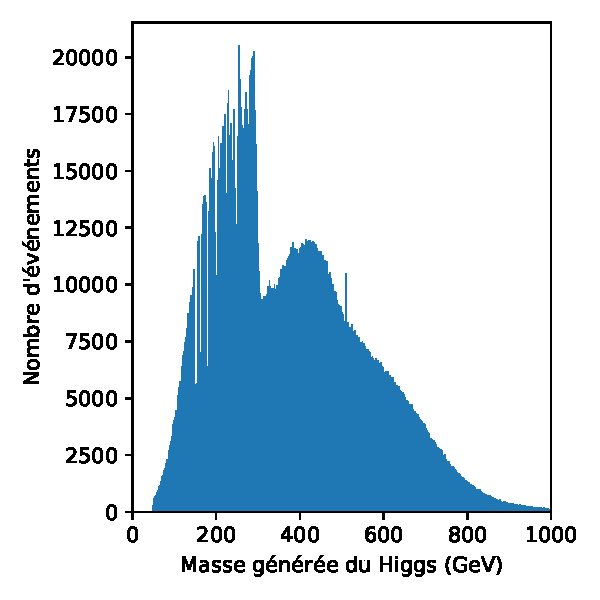
\includegraphics[width=.45\textwidth]{\PhDthesisdir/plots_and_images/my_plots/ML/from_ML_plots/FastSim_NanoAOD_to_NN/ALL_PU2017/plots_Htt_merged_NanoAODSIM_ALL_PU2017-DeepTau/distribution-inclusive-Higgs_mass_gen-raw-all_events.pdf}}
\hfill
\subcaptionbox{Distribution pondérée pour les événements d'entraînement.\label{subfig-distribution-inclusive-Higgs_mass_gen-weighted-is_train}}[0.45\textwidth]
{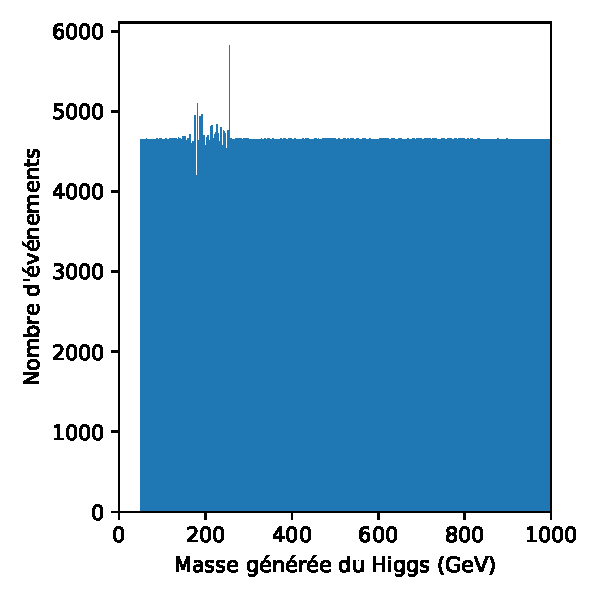
\includegraphics[width=.45\textwidth]{\PhDthesisdir/plots_and_images/my_plots/ML/from_ML_plots/FastSim_NanoAOD_to_NN/ALL_PU2017/plots_Htt_merged_NanoAODSIM_ALL_PU2017-DeepTau/distribution-inclusive-Higgs_mass_gen-weighted-is_train.pdf}}

\caption[Distributions de la masse générée de \higgsML.]{Distributions de la masse générée de \higgsML.}
\label{fig-distribution-inclusive-Higgs_mass_gen-raw-all_events}
\end{figure}